\documentclass{beamer}
\usepackage[french]{babel}
\usepackage[utf8]{inputenc}
\usepackage[T1]{fontenc}
\usetheme{metropolis}

\title{Systèmes de Gestion de Versions}
\date{\today}
\author{David Ananda, Pierre-Louis Sergent, Matthieu Kirschleger, Bruno Inec}
\institute{IUT informatique Lyon1}

\begin{document}
  \maketitle

  \begin{frame}{Table des matières I}
    \tableofcontents[sections={1}]
      \framebreak
    \tableofcontents[sections={2}]
  \end{frame}
  \begin{frame}{Table des matières II}
    \tableofcontents[sections={3}]
  \end{frame}

  \section{Histoire}
\subsection{SCCS \& RCS}
\begin{frame}{SCCS \& RCS}
  \begin{columns}[T]

    \begin{column}{.5\textwidth}
      GNU SCCS (Source Code Control System), 1972
      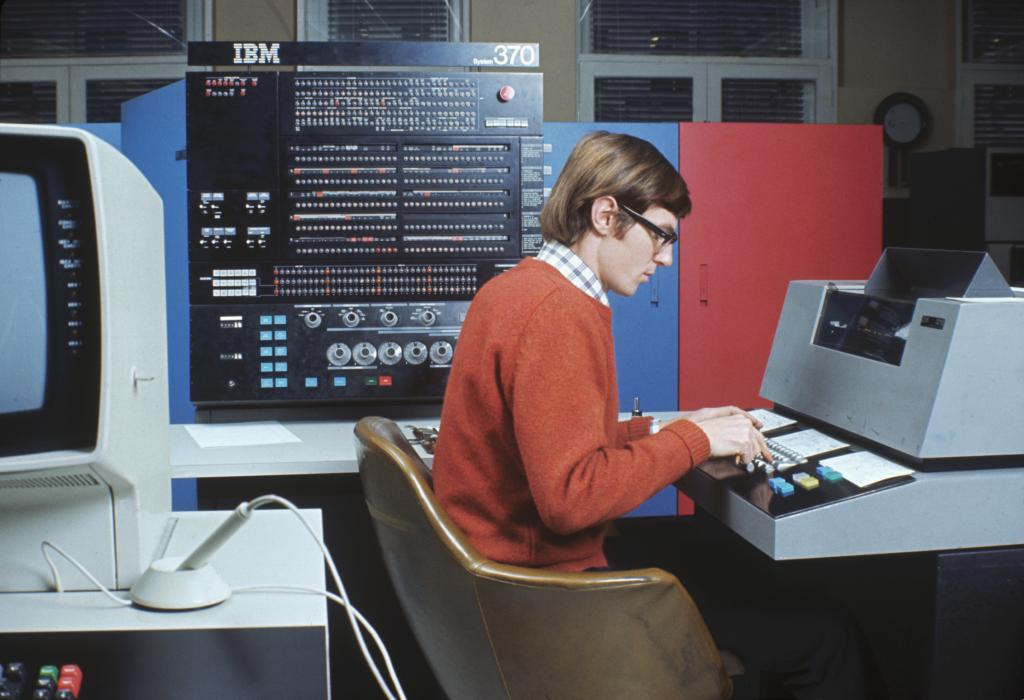
\includegraphics[width=\textwidth]{./ibm-system-370.png}
    \end{column}

    \begin{column}{.5\textwidth}
      GNU RCS (Revision Control System), 1982
      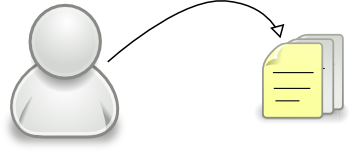
\includegraphics[width=\textwidth]{./rcs-model.png}
    \end{column}

  \end{columns}
\end{frame}

\subsection{CVS \& SVN}
\begin{frame}{CVS \& SVN}
  \begin{columns}[T]

    \begin{column}{.5\textwidth}
      CVS (Concurrent Versions System), 1990
      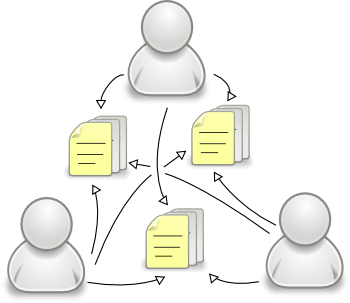
\includegraphics[width=\textwidth]{./cvs-model.png}
    \end{column}

    \begin{column}{.5\textwidth}
      SVN (Subversion), 2000
      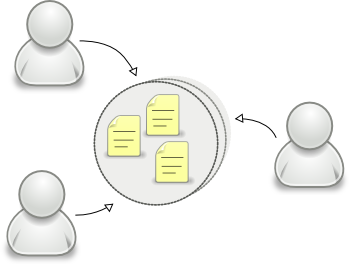
\includegraphics[width=\textwidth]{./svn-model.png}
    \end{column}

  \end{columns}
\end{frame}

\subsection{Git, Mercurial \& Bazaar}
\begin{frame}{Git, Mercurial \& Bazaar}
  \begin{columns}[T]

    \begin{column}{.5\textwidth}
      Git, 2005

      Mercurial, 2005

      GNU Bazaar, 2005
    \end{column}

    \begin{column}{.5\textwidth}
      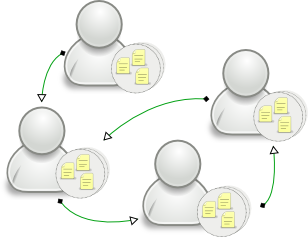
\includegraphics[width=\textwidth]{./hg-model.png}
    \end{column}

  \end{columns}
\end{frame}

  \section{Décentralisé vs Centralisé}
\subsection{Principe de base d'un VCS}
\begin{frame}{Principe de base d'un VCS}
  Gérer le mécanisme lecture-fusion-écriture
  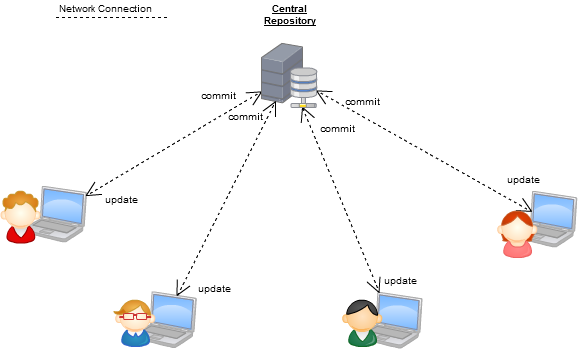
\includegraphics[width=\textwidth]{./diapo1.png}
\end{frame}

\subsection{Gestionnaire de versions centralisée CVCS}
\begin{frame}{Gestionnaire de versions centralisée CVCS}
  \begin{columns}[T]

    \begin{column}{.6\textwidth}
      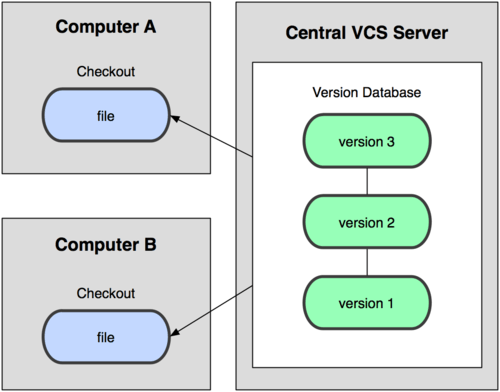
\includegraphics[width=\textwidth]{./CVCS.png}
    \end{column}

    \begin{column}{.4\textwidth}
      \begin{itemize}
        \item{Un seul dépôt de référence (serveur)}
        \item{Les utilisateurs travaillent sur une copie}
      \end{itemize}
    \end{column}

  \end{columns}
\end{frame}

\begin{frame}{Gestionnaire de versions centralisée CVCS}
  Qualités:
  \begin{itemize}
    \item{technologie éprouvée}
    \item{largement disponible}
    \item{sécurisé}
  \end{itemize}

  Défauts:
  \begin{itemize}
    \item{échange entre les dépôts impossible}
    \item{échange entre les copies locales impossible}
    \item{travail hors connexion impossible}
    \item{dépendant du serveur}
  \end{itemize}
\end{frame}

\subsection{Présentation SVN}
\begin{frame}{Présentation SVN}
  Serveur centralisé et unique:
  \begin{itemize}
      \item{les fichiers de reférences (le dépôt ou repository)}
      \item{un logiciel serveur SVN tournant en tâche de fond}
  \end{itemize}

  Postes clients:
  \begin{itemize}
      \item{copie locale du repo, éventuellement modifié}
      \item{logiciel client permettant la synchronisation manuelle et/ou
            automatisée entre chaque client et le serveur de ref}
  \end{itemize}
  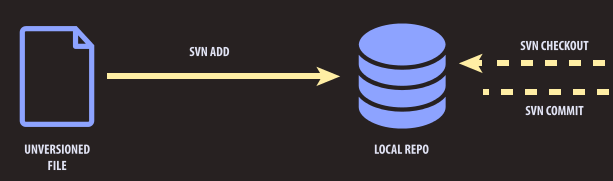
\includegraphics[width=\textwidth]{./svn1.png}
\end{frame}

\subsection{Gestionnaire de versions décentralisée DVCS}
\begin{frame}{Gestionnaire de versions décentralisée DVCS}
  \begin{columns}[T]

    \begin{column}{.6\textwidth}
      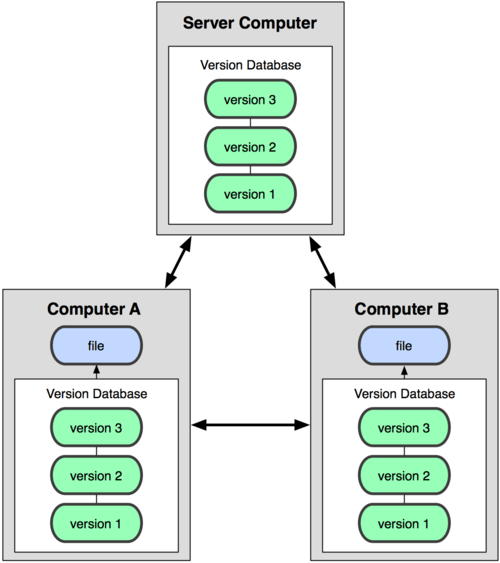
\includegraphics[width=\textwidth]{./DVCS.png}
    \end{column}

    \begin{column}{.4\textwidth}
      \begin{itemize}
        \item{Dépôt propre à chaque développeur}
        \item{Copie propre à chaque développeur}
      \end{itemize}
    \end{column}

  \end{columns}
\end{frame}

\begin{frame}{Gestionnaire de versions centralisée CVCS}
  Qualités:
  \begin{itemize}
    \item{communication possible entre les dépôts}
    \item{possibilité de mettre en place un dépôt central (serveur)}
    \item{travail hors connexion possible}
    \item{indépendant du serveur}
    \item{gestion des branches}
    \item{gestion des merges}
  \end{itemize}

  Défauts:
  \begin{itemize}
    \item{complexité (Git)}
  \end{itemize}
\end{frame}

  \section{Git vs Mercurial}
\subsection{Format du dépôt}
\begin{frame}{Format du dépôt}
  \begin{columns}[T]

    \begin{column}{.5\textwidth}
    \textsc{Mercurial}

    \vspace{\baselineskip}

    A tout misé sur les logs en append-only, optimiser la recherche sur le
    disque de nos machines
    \end{column}

    \begin{column}{.5\textwidth}
    \textsc{Git}

    \vspace{\baselineskip}

    Stocke chaque commit/fichier dans un simple dépôt de ‘hash’ de documents,
    chaque commit finira dans ce dépôt comme une entité séparée
    \end{column}

  \end{columns}
\end{frame}

\subsection{Réécrire l'historique}
\begin{frame}{Réécrire l'historique}
  \begin{columns}[T]

    \begin{column}{.5\textwidth}
     \textsc{Mercurial}

      \begin{itemize}
        \item{Édition difficile des commits passés or il est plus facile de
              voir les chgmts en examinant l’histoire par les commits}
        \item{Mercurial Queus permet d’empiler des pré-commits de sorte à
              pouvoir les réorganiser jusqu’à votre commit final}
        \item{Extension  équivalente de “interactive rebase” = “histedit” →
              append-only → génère un fichier de sauvegarde externe →
              problèmes: comment analyser les modifications de cette
              sauvegarde? Pendant combien de temps peut-on sauvegarder les
              sauvegardes}
      \end{itemize}
    \end{column}

    \begin{column}{.5\textwidth}
      \textsc{Git}

      \begin{itemize}
        \item{Il est facile de « remonter le temps » pour éditer les commits
              précédents si nécessaire → les logs de commit Git peuvent devenir
              des récits soigneusement élaborés (voir Mercurial Queus)}
        \item{Vous arriverez au moment où vous avez besoin de faire un
              changement dans votre historique de commits; vous n’aurez
              vraiment qu’une seule chose à savoir: « interactive rebase »
              (git rebase -i) → permet de modifier l’histoire de Git comme on
              veut}
        \item{Git ne détruit pas les objets ayant une référence, pour arrêter
              le « garbage collector » de Git et retrouver une sauvegarde →
              appliquer un tag pour référence future → ce sont des commits sans
              branches}
      \end{itemize}
    \end{column}

  \end{columns}
\end{frame}

\subsection{Les branches}
\begin{frame}{Les branches}
  \begin{columns}[T]

    \begin{column}{.5\textwidth}
      \textsc{Git}

      \begin{itemize}
        \item{Namespace du serveur indique clairement qui est qui}
      \end{itemize}
    \end{column}

    \begin{column}{.5\textwidth}
      \textsc{Mercurial}

      \begin{itemize}
        \item{Extension Bookmark → clone direct des branches Git, au début on
              pouvait pas faire le push des bookmarks sur le serveur}
        \item{Problème: les bookmarks partagent le même namespace}
      \end{itemize}
    \end{column}

  \end{columns}
\end{frame}

\subsection{Staging (zone de transit)}
\begin{frame}{Staging (zone de transit)}
  \begin{columns}[T]

    \begin{column}{.5\textwidth}
      \textsc{Git}
      \begin{itemize}
        \item{Tout ce qu’on ajoute à un commit passe par cette zone de transit:
              commande “git add” → appelée aussi index}
        \item{On ajoute des modifications, pas aux fichiers eux-mêmes,
              mais au reflog}
      \end{itemize}
    \end{column}

    \begin{column}{.5\textwidth}
      \textsc{Mercurial}
      \begin{itemize}
        \item{Extension Record}
        \item{Doit copier les modifications ‘dans un emplacement temporaire →
              mettre à jour les fichiers de stockage, commit → enfin annuler
              les modifications}
        \item{Erreur = on recommence tout}
      \end{itemize}
    \end{column}

  \end{columns}
\end{frame}


  \begin{frame}{Conclusion}
    \Large
    In conclusion.

    Save lives, use Git or Mercurial. (no more google drive for code sharing...)
  \end{frame}
\end{document}

